\documentclass{ctexart}
\usepackage{graphicx} % Required for inserting images
\usepackage{amsmath}
\usepackage{booktabs}
\usepackage[left=2.5cm,right=2.5cm,top=2.5cm,bottom=2.5cm]{geometry}
\begin{document}
\section{实验目的}
(1)掌握判断三相电源相序方法;

(2)三相照明电路设计与实现;

(3)三相异步电机控制电路设计。

\section{预习要求}
\subsection{预习相序判断的方法,并简述原理}
相序是指三相交流电的幅值和相位关系,即它们的顺序。在电力系统中,三相交流电的幅值和相位应该是平衡的,否则会导致系统不稳定。相序判断就是确定三相交流电的幅值和相位关系的过程。

相序判断的方法主要有两种:一是使用三个电流表分别测量三相电流的幅值和相位,然后根据测量结果计算相序;二是使用三个电压表分别测量三相电压的幅值和相位,然后根据测量结果计算相序。

原理是:根据三相交流电的数学模型,三相交流电的瞬时值可以用三个正弦函数表示,即
\begin{equation}
\begin{cases}
    i_A(t)=I_m\sin (\omega t)\\
    i_B(t)=I_m\sin (\omega t + 120 ^{\circ})\\
    i_C(t)=I_m\sin (\omega t + 240 ^{\circ})
\end{cases} 
\end{equation}
其中$i_A$、$i_B$、$i_C$分别为三相电流的幅值,$\omega$为角频率,$\varphi$为初相位。因此,如果三相交流电的幅值和相位关系与上述式子相符,则说明相序为正序。否则,相序为逆序或零序。

具体来说,可以通过实验方法测得相序。利用示波器的双通道显示,两两测量相邻两个通道之间的相位差,就可以判断相序。
\subsection{预习三相异步电动机控制电路相关知识}
三相异步电动机的控制电路包括多种类型,例如正转控制电路、反转控制电路、点动控制电路、自锁正转控制电路、接触器联锁的正反转控制电路等。

其中,正转控制电路包括简单的正转控制电路和点动正转控制电路。简单的正转控制电路只需一个手动开关,操作简单但功能有限。点动正转控制电路则通过按钮和接触器来实现,按钮的按下使接触器线圈得电,电动机启动;松开按钮,接触器线圈失电,电动机停止。

反转控制电路可以通过改变电源相序来实现,也可以使用反转控制按钮和接触器来实现。

自锁正转控制电路在点动正转控制电路的基础上增加了接触器辅助触头,使其具有自锁功能,能实现欠电压和失电压保护。

接触器联锁的正反转控制电路使用两个接触器,通过它们的联锁实现正反转互锁,避免电源短路。
\subsection{设计实验内容(1),并记录仿真结果(截图)}
设计图如图\ref{fig:双联双控开关电路}所示
\begin{figure}[!ht]
    \centering
    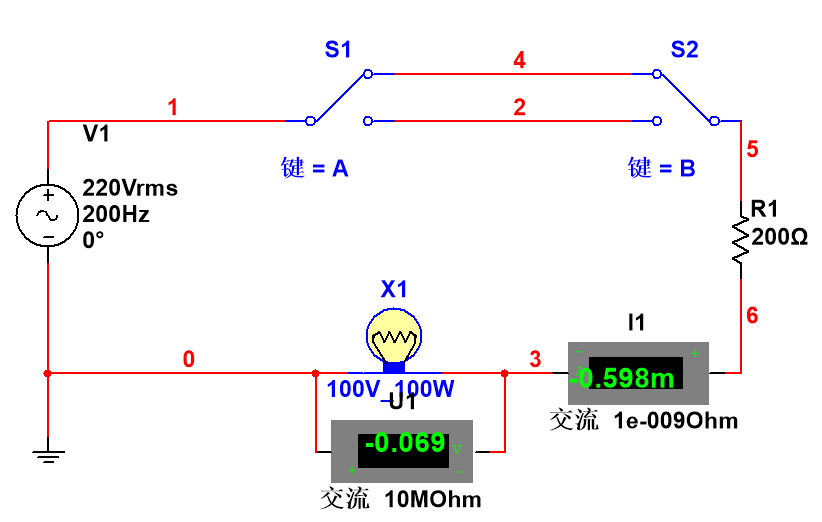
\includegraphics{pic/双联双控开关电路.png}
    \caption{双联双控开关电路}
    \label{fig:双联双控开关电路}
\end{figure}
\subsection{试分析正反转控制电路原理}
合上电源开关Q,,按下正转按钮$SB_F$,这时正转回路被供电,线圈$KM_F$启动,带动对应的开关$KM_F$按下,连通电动机电路,且此时$SB_F$断开也没有关系,因为其下方的$KM_F$已经接通。按下$SB_1$断开电路,线圈断电,$KM_F$弹开,电动机电路断开,反转控制电路同理
\section{实验内容}
\section{实验仪器}
\section{实验总结}
\section{参考文献}

\end{document}
